\documentclass[withoutpreface,bwprint]{apmcmthesis}
\tihao{B}
\baominghao{apmcm2699001}
\usepackage{amsmath,amssymb,booktabs,longtable,array,graphicx,listings}
\lstset{basicstyle=\ttfamily\scriptsize,columns=fullflexible,frame=none,aboveskip=0.4em,belowskip=0.4em}
\emergencystretch=1.5em
\begin{document}
\thispagestyle{empty}
\begin{abstract}
\begin{center}
{\Large\bfseries Desulfurized Ash in Cotton-Stalk Pyrolysis:\\ Compositional Signal, Species Tiers, and a Prediction Envelope}
\end{center}
\vspace{0.4em}

\textbf{Background and Task} Co-pyrolysing cotton stalk with desulfurized fly ash (DFA) is promoted as a way to upgrade the gas, yet the two annexes of Problem~B report four product yields that must sum to one and a separate gas table in a different unit, with a declared relative error near 5 percent on every cell. We ask five questions: whether DFA changes the product distribution and by how much, how each gas species responds, whether cellooligosaccharide (CE) and lignin (LG) differ at equal ash loading, which mechanism and kinetics are consistent with those responses, and what can be predicted at an untried loading. The annexes sample the three mixtures on grids that only partly coincide, so every comparison is built on the levels they share.

\textbf{Modeling Framework} Because the four yields are one composition, the analysis works in isometric log-ratio (ILR) coordinates on a three-part simplex instead of four independent regressions. Question~1 is answered by an ILR linear model in the ash mass fraction. Question~2 adds a species-level, noise-calibrated tiering and a mole-fraction bridge between the two annexes. Question~3 turns the fit into a paired contrast at equal ash level. Question~4 combines a centred log-selectivity, a gas-phase carbon account, and an isothermal iso-conversion ridge. Question~5 propagates the fitted residual through a Monte-Carlo prediction envelope and checks it by leave-one-out.

\textbf{Results per Question} DFA reshapes the distribution rather than diluting it: on a dry-ash-free basis the ash cannot lower a yield mechanically, yet for cotton stalk tar falls by -37.7 percent between the zero-ash and the richest level, while the dominant lignin product stays inside its noise floor. The strongest gas signal is hydrogen in cotton stalk, whose span is 14.47 times its own floor. At equal ash level CE and LG separate most sharply on char, with a mean gap of -33.27 points, and water is the only product that changes sign. The gas-phase carbon account falls by 77.2 percent along the CE series, which links the yield shifts to a carbon-partition change. The cotton-stalk leave-one-out error is 5.50 percent, the smallest of the three mixtures.

\textbf{Validation and Limitation} Mass closure holds to machine precision, and every reported number is recomputed from the stored result files. A perturbation audit of the fitted parameters and the query points leaves a single headline reversal, 6.67 percent of the feasible model runs. The main limitation is that neither annex reports the pyrolysis temperature, so the kinetics reduce to an iso-conversion ridge and no rate law is identified; the CE and LG series also show a lack-of-fit ratio of 3.42 or more, which marks their predictions as trend-only.

\keywords{Compositional data; Isometric log-ratio regression; Noise-calibrated species tiering; Paired contrast at equal ash level; Selectivity and carbon accounting; Monte-Carlo prediction envelope}
\end{abstract}

\newpage
\setcounter{tocdepth}{1}
\tableofcontents
\newpage
\pagestyle{mainmatterstyle}
\setcounter{page}{1}

\section{Introduction}
\subsection{Background}
Cotton stalk is one of the largest dry agricultural residues in the cotton belt, and pyrolysis converts it into a solid char, a condensable tar, water, and a non-condensable gas whose hydrogen content determines its value as a fuel or a reducing agent \cite{Bridgwater2012,Czernik2004}. Ash-rich industrial residues such as desulfurized fly ash (DFA) are abundant, and their lime and sulfate content makes them plausible catalysts for tar cracking and carbon dioxide uptake \cite{Sutton2001,Blamey2010}. Co-processing therefore looks attractive, but it raises a measurement question that a yield table alone can answer only if the table is read correctly: the four product yields are percentages of one dry-ash-free mass, so they are a composition with three degrees of freedom, not four independent responses.

\subsection{Restatement of the Problems}
Write $a$ for the DFA mass charged per 100\,g of dry biomass, $r=a/100$, and $w=r/(1+r)=a/(100+a)$ for the ash mass fraction of the feed. For mixture $c\in\{\mathrm{CS},\mathrm{CE},\mathrm{LG}\}$ and product $p\in\{\mathrm{Tar},\mathrm{Water},\mathrm{Char},\mathrm{Syngas}\}$, let $y_p^{(c)}$ be the yield in wt.\% (daf), and for gas species $g$ let $z_g^{(c)}$ be the yield in mL/g (daf). The five tasks are:
\begin{enumerate}
\item estimate how each $y_p^{(c)}$ responds to $w$, and decide for each product whether the response exceeds the declared experimental error;
\item describe how each $z_g^{(c)}$ responds to $w$, and present the gas composition in a form that is comparable across mixtures;
\item compare CE with LG at the same ash level, decide which product and gas gaps are real, and explain the pattern;
\item propose a reaction mechanism consistent with Questions~1--3, and determine which kinetic parameters the data can and cannot identify;
\item predict $y_p^{(c)}$ on a requested ash grid for a mixture with no further experiments, with an uncertainty statement.
\end{enumerate}

\subsection{Our Work}
This paper delivers five linked results. (i) An ILR linear model of the full composition, with a noise-calibrated decision for all twelve product--mixture combinations; tar and water respond in every mixture, char responds only through a derived column. (ii) A species-level tiering by absolute span and a mole-fraction bridge that shows the gas annex and the product annex are not the same measurement. (iii) A paired CE--LG contrast on eight product levels and five gas levels, which separates the feedstocks on tar, char, hydrogen, carbon dioxide, and methane but not on water. (iv) A mechanism reading in three independent signatures, and an honest kinetic result: an iso-conversion ridge, not a rate law. (v) A prediction table on a seven-level grid with 5--95\% intervals, whose reliability is established by leave-one-out rather than asserted. Every number printed below is recomputed from \texttt{data/results\_*.json} by \texttt{code/verify\_numbers.py}; the 547 stored claims and their provenance are itemised in that script.

\section{Problem Analysis}
Three features of the data decide the whole modelling strategy.

\textbf{The response is a composition.} Each Annex~I row sums to 100 by construction (the largest observed deviation is $1.4\times10^{-14}$), so the four yields carry three degrees of freedom. Fitting four separate regressions would count the same information twice and would produce coefficients that cannot be compared across mixtures, a defect of ordinary univariate treatment of shares that has been documented repeatedly \cite{Aitchison1982,Filzmoser2009}. Working in log-ratio coordinates removes both defects and makes the coefficients interpretable as elasticities: the fitted model predicts shares, and the inverse transform returns a composition that sums to one exactly \cite{Egozcue2003,Pawlowsky2011}.

\textbf{The dry-ash-free basis removes dilution.} Because $y_p$ is expressed per gram of dry ash-free biomass, adding inert ash cannot lower a yield by replacing fuel with ash. Any change in $y_p$ is therefore chemical, or an artefact of the normalisation, and the paper is careful to distinguish the two. This is why the phrase ``the ash dilutes the products'' is not available as an explanation here, and why the observed tar loss in cotton stalk is a statement about chemistry rather than about mass balance.

\textbf{The declared error is the object of inference.} Every cell carries a relative error near 5\%, so a smooth curve drawn through four points is not evidence of a trend. Three thresholds are therefore defined and kept separate: a step threshold for adjacent levels, a difference threshold for the paired CE--LG contrast, and a trend threshold for a whole series. They answer different questions and are never substituted for one another. A ratio of span to threshold above one is reported as a signal, and the denominator is always named, because the same word ``significant'' would otherwise mean three different things in three sections.

Two secondary features matter as well. First, the two annexes use different units (mass fraction against volume per gram), so a bridge is needed before they can be discussed together; the bridge is a diagnostic, not a correction. Second, three product columns are stored as formulas rather than measurements (CS syngas, CE char, and LG tar), which makes their fitted responses partly arithmetic; these cells are flagged wherever they are used.

\section{Assumptions and Justifications}
\begin{enumerate}
\item \textbf{Independent 5\% relative error.} Each reported cell is treated as a measurement with independent relative error $\varepsilon=0.05$; this is the only error statement the problem supplies, and no replicate exists to estimate it. Used by every threshold in Sections~\ref{sec:q1}--\ref{sec:q5} and by the surrogate noise simulation.
\item \textbf{Exact closure.} The four product yields of a row sum to unity, so the composition lives on the simplex. Verified on all rows (maximum deviation $1.4\times10^{-14}$); used by the ILR transform.
\item \textbf{Uniform preparation precision.} Columns within one annex were measured with the same precision, so a single $\varepsilon$ applies to all of them. Structural, not testable from the annex; used when pooling residuals.
\item \textbf{Smooth, linear response in ILR coordinates.} Over the sampled ash range each ILR coordinate is linear in $w$. Tested by a lack-of-fit ratio against the surrogate noise floor; it holds for CS and is rejected for CE and LG, which are then reported as trend descriptions only.
\item \textbf{Comparable pyrolysis conditions across feedstocks.} CE and LG were pyrolysed under the same conditions as CS, so a CE--LG contrast at equal ash level is a feedstock contrast. Partly supported by the shared level grid; used by Section~\ref{sec:q3} and by the ranking of mechanisms in Section~\ref{sec:q4}.
\item \textbf{The gas annex measures relative composition only.} Annex~II volumes are used to compare species and mixtures, never to close a mass balance against Annex~I. Tested by the bridge ratio, whose range shows the two annexes do not report the same quantity.
\item \textbf{A reporting threshold of 5\,mL/g (daf) separates major from minor species.} This is a presentation convention, not a physical constant; the interval of thresholds that preserves every tier is reported, and the sensitivity of the tiers is measured.
\item \textbf{The isothermal endpoint identifies only the product $k(T)t$.} With one temperature and one holding time, the pre-exponential factor and the activation energy cannot be separated. Used in Section~\ref{sec:q4}: an iso-conversion ridge is reported instead of a point estimate.
\item \textbf{Stability is assessed by perturbation, not replication.} With no replicate runs, stability is measured by perturbing inputs, thresholds, and query points, and by leave-one-out refitting. Used in Sections~\ref{sec:q5} and~\ref{sec:sens}.
\item \textbf{The prediction grid lies inside the observed support.} All seven requested ash levels fall between the smallest and largest calibrated levels of each mixture, so the exercise is interpolation; the boundary check confirms this and flags the levels that sit on the support edge.
\end{enumerate}

\section{Notations and Data}
\subsection{Notations}
Symbols are listed with their ranges in Appendix~A. In the body, $w$ is the ash mass fraction of the feed, $S_p=y_p/100$ is a product share, $z_g$ is a gas yield, $\varphi_g$ is a gas mole fraction, $\gamma_p$ is a centred log-selectivity, $\beta$ is the annex bridge ratio, $n_C$ is gas-phase carbon, and $k$, $A$, $E_a$, $n$, $f(\alpha)$ are kinetic quantities.

\subsection{Data Sources and Structure}
Annex~I contains 25 product rows (CS 9, CE 8, LG 8) and four product columns, 100 cells in all; Annex~II contains 16 gas rows (CS 6, CE 5, LG 5) and 54 + 25 + 25 = 104 gas cells, with species counts 9, 5, 5. The two grids are nested rather than identical: Annex~I uses nine levels for CS and eight for CE and LG, Annex~II six and five. The shared product levels number eight for the CE--LG contrast, and the shared gas levels number five. The level $100/100$ means a DFA mass fraction of 50.0000\%, not pure ash; the mapping $w=r/(1+r)$ is applied before any fitting, and the unequal spacing of $r$ (steps of 10 up to 60, then 20) is one reason the response is modelled in $w$ rather than in $r$. Both annexes are used exactly as published in the problem statement \cite{ProblemB2023}; no value is edited, imputed, or rescaled.

\subsection{Cleaning and Cross-Checks}
No cell is missing. Three product columns are derived by subtraction (CS syngas, CE char, LG tar; 24 cells), and they are marked in every table and every claim. Closure holds to $1.4\times10^{-14}$. A surrogate experiment draws 4000 compositions with independent 5\% multiplicative noise, recloses them, and transforms them by ILR; the standard deviation of the transformed surrogate is the noise floor used in Section~\ref{sec:q1}. Its value, 0.0502 on the CS grid and 0.0501 on the CE and LG grids, is close to the analytic expectation for a four-part composition and confirms that the declared error and the fitted residual are on the same scale.

\subsection{Rationality of the Comparison}
The declared 5\% is a property of the measurement, not an accuracy target for the model; a model whose residual is smaller than the floor is not ``better'', it is merely consistent. Conversely, a fitted residual above the floor indicates lack of fit, not precision. This asymmetry is used explicitly: CS has a residual below the floor, so its linear ILR model is accepted; CE and LG have residuals above it, so their models are demoted to trend descriptions. The three derived columns are treated as arithmetic consequences of the other three, and a response that appears only in a derived column is never promoted to a chemical finding.

\section{Question 1: Product Yields against Ash Loading}
\label{sec:q1}
\subsection{Mechanism and Rationale}
DFA brings lime, sulfate, and silica into the bed. Lime is a carbon dioxide sorbent and a tar-cracking contact; sulfate can act as an oxygen carrier; silica is largely inert \cite{Sutton2001,Blamey2010}. Two responses are therefore plausible on chemical grounds: tar should fall as volatiles are cracked, and gas should rise as the fragments become non-condensable. Char is expected to be the least responsive product, because the dry-ash-free basis already removes the inert fraction and because char is the residue that the ash does not consume. The data are asked whether these expectations survive the noise floor, not whether they are plausible.

\subsection{Model}
The ash fraction is
\begin{equation}
r=\frac{a}{100},\qquad w=\frac{r}{1+r}=\frac{a}{100+a},
\label{eq:w}
\end{equation}
and the composition is
\begin{equation}
S_p=\frac{y_p}{100},\qquad \sum_{p}S_p=1 .
\label{eq:S}
\end{equation}
With four parts, a Helmert contrast basis gives three orthonormal coordinates,
\begin{equation}
v_1=\frac{\ln S_1-\ln S_2}{\sqrt{2}},\quad
v_2=\frac{\ln S_1+\ln S_2-2\ln S_3}{\sqrt{6}},\quad
v_3=\frac{\ln S_1+\ln S_2+\ln S_3-3\ln S_4}{\sqrt{12}},
\label{eq:ilr}
\end{equation}
which is the isometric log-ratio transform of \cite{Egozcue2003} in the Helmert form used by the \texttt{compositions} package \cite{Boogaart2008}; each coordinate is modelled as
\begin{equation}
v_j=\beta_{j0}+\beta_{j1}w+e_j,\qquad j=1,2,3,
\label{eq:fit}
\end{equation}
and the composition is recovered from a prediction $\hat v$ by
\begin{equation}
u_p=\sum_{j=1}^{3}\hat v_j V_{jp},\qquad
\hat S_p=\frac{\exp u_p}{\sum_{q}\exp u_q},\qquad \sum_p \hat S_p=1 .
\label{eq:inv}
\end{equation}
The fitted slopes also define the selectivity used in Section~\ref{sec:q4}: with $b_p=\mathrm{d}\ln S_p/\mathrm{d}w$ obtained by regressing $\ln S_p$ on $w$,
\begin{equation}
\gamma_p=b_p-\frac{1}{4}\sum_q b_q,\qquad \sum_p\gamma_p=0 .
\label{eq:gamma}
\end{equation}
Three thresholds are used, all with the declared $\varepsilon=0.05$ and a factor two for a two-standard-deviation band:
\begin{align}
\tau_{s}(k)&=2\varepsilon\max\{|y_k|,|y_{k+1}|\},\label{eq:step}\\
\tau_{T}&=2\varepsilon\,\overline{|y|},\label{eq:trend}\\
\tau_{D}&=2\varepsilon\sqrt{y_a^2+y_b^2}.\label{eq:diff}
\end{align}
A series is called a trend when its end-to-end span exceeds $\tau_{T}$; a step is called resolved when its change exceeds $\tau_{s}$; a paired gap is called real when it exceeds $\tau_{D}$.

\subsection{Results}
Table~\ref{tab:q1} reports the twelve product--mixture combinations, Figure~\ref{fig:q1yield} the fitted curves, and Figure~\ref{fig:q1span} the span-to-floor ratios. Fitting is a six-parameter linear least squares per mixture on 27 (CS) or 24 (CE, LG) observations; the three-coordinate fit takes a median of 189.7\,ms in the reference implementation, so the cost is negligible and the algorithm is ordinary least squares on a $27\times2$ design.

\begin{table}[htbp]\centering
\caption{Product response to ash loading. First and last are the yields at the first and last stored level of each mixture (CS: $w=0$ to $0.50$; CE and LG: $w=0.0909$ to $0.50$). The span is $\max y-\min y$, $\tau$ is the trend threshold of Eq.~\eqref{eq:trend}, and the last column gives the span-to-floor ratio. A dagger marks a column stored as a formula rather than measured.}
\label{tab:q1}
{\small\setlength{\tabcolsep}{1.7pt}
\begin{tabular}{@{}llrrrrrrl@{}}
\toprule
Mixture & Product & First & Last & $\Delta y$ & $\Delta\%$ & Span & Span$/\tau$ & Call\\
\midrule
CS & Tar & 19.46 & 12.13 & -7.33 & -37.7 & 7.33 & 5.04 & trend\\
CS & Water & 26.84 & 31.02 & 4.18 & 15.6 & 4.18 & 1.45 & trend\\
CS & Char & 29.21 & 29.87 & 0.66 & 2.26 & 0.76 & 0.259 & flat\\
CS & Syngas$^{\dagger}$ & 24.49 & 26.98 & 2.49 & 10.2 & 3.96 & 1.46 & trend\\
CE & Tar & 34.42 & 45.28 & 10.86 & 31.6 & 10.86 & 2.58 & trend\\
CE & Water & 27.42 & 16.14 & -11.28 & -41.1 & 11.28 & 5.86 & trend\\
CE & Char$^{\dagger}$ & 21.43 & 24.61 & 3.18 & 14.8 & 3.48 & 1.45 & trend\\
CE & Syngas & 16.73 & 13.97 & -2.76 & -16.5 & 3.98 & 2.73 & trend\\
LG & Tar$^{\dagger}$ & 18.06 & 8.19 & -9.87 & -54.7 & 9.87 & 8.73 & trend\\
LG & Water & 15.3 & 23.69 & 8.39 & 54.8 & 8.39 & 4.11 & trend\\
LG & Char & 58.17 & 57.43 & -0.74 & -1.27 & 1.19 & 0.208 & flat\\
LG & Syngas & 8.47 & 10.69 & 2.22 & 26.2 & 3.41 & 3.12 & trend\\
\bottomrule
\end{tabular}}
\end{table}

\begin{figure}[htbp]\centering
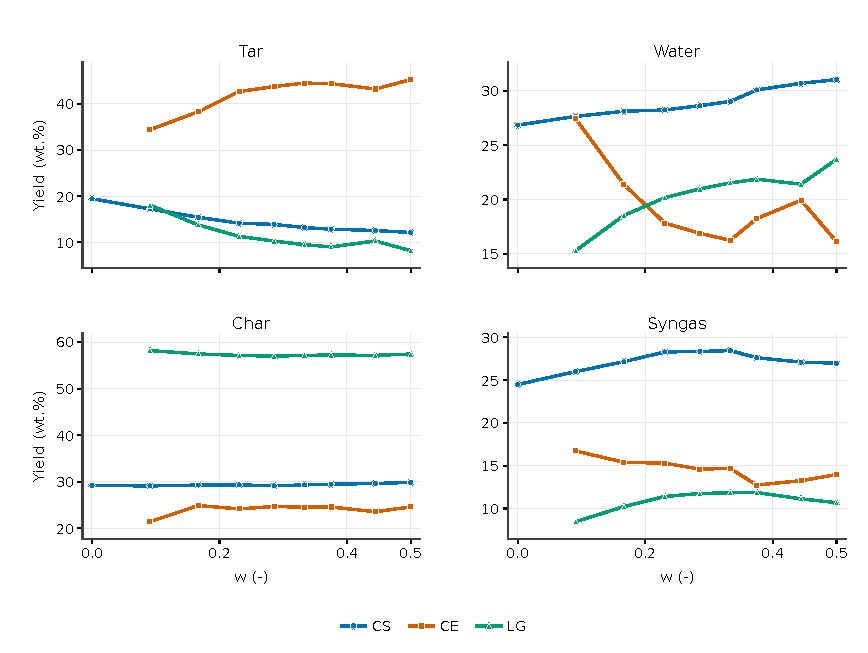
\includegraphics[width=\linewidth]{figures/fig01_q1_product_yields.pdf}
\par\vspace{1pt}{\footnotesize\raggedright% generated by code/make_figures.py -- do not edit
Q1: product yields from stored Annex I levels

source: data/results\_q1.json; generator: code/make\_figures.py
\par}
\caption{Product yields (wt.\%) of the three mixtures against the ash-to-biomass ratio $w$: Tar, Water, Char and Syngas. Each panel keeps its own yield axis; colour and marker identify CS, CE and LG, and the lines pass through the stored Annex~I levels.}
\label{fig:q1yield}
\end{figure}

\begin{figure}[htbp]\centering
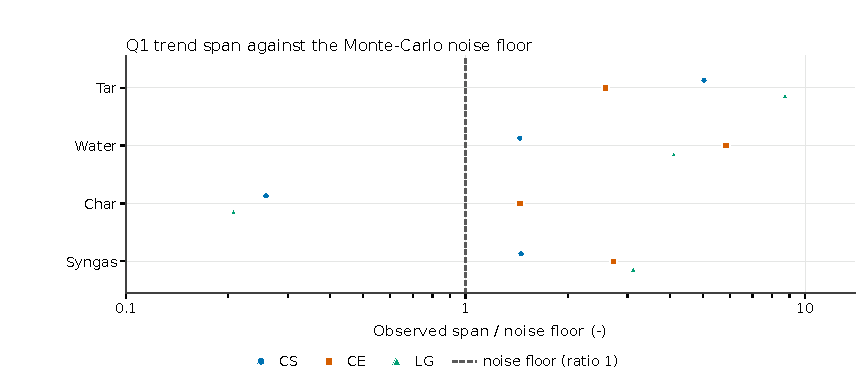
\includegraphics[width=\linewidth]{figures/fig02_q1_span_noise.pdf}
\par\vspace{1pt}{\footnotesize\raggedright% generated by code/make_figures.py -- do not edit
Q1: observed span against the surrogate noise floor

source: data/results\_q1.json; generator: code/make\_figures.py
\par}
\caption{Observed end-to-end span of each product series divided by the Monte-Carlo noise floor, on a log axis; the dashed line at 1 is the noise floor itself. Points left of the line move less across the whole level range than the surrogate noise does.}
\label{fig:q1span}
\end{figure}

Tar falls in cotton stalk (-37.7\%, a span of 7.33 against a floor of 1.45) and in lignin (-54.7\%, span 9.87 against 1.13), but rises in CE (31.6\%) and in the CE series the rise is 10.86 against a floor of 4.21. Water moves the other way in CS (+15.6\%) and LG (+54.8\%) and falls sharply in CE (-41.1\%). Char is flat in CS (ratio 0.259) and in LG (ratio 0.208) but rises by 14.8\% in CE; that rise belongs to a derived column, so the chemical claim is withheld. Syngas rises in CS (+10.2\%) and LG (+26.2\%) and falls in CE (-16.5\%). The answer to ``is DFA significant'' is therefore: for tar and for water, yes, in every mixture; for syngas, yes in two of three; for char, no measured column moves outside its floor, and the single apparent char response is arithmetic.

\subsection{A Counter-Intuitive Reading and Validation}
Two results contradict the intuitive picture. First, the largest product in lignin, char at 58.17\,wt.\%, is the one product that does not respond (span 1.19 against a floor of 5.73), while tar, which is a fifth of the mass, changes by more than half. Second, the CS syngas series is a trend that contains no resolved step: its span clears the trend floor by a factor of 1.46 while all eight adjacent changes sit inside their step thresholds. A reader who only tested steps would call this series flat; a reader who only tested ends would miss that the movement is spread evenly rather than concentrated.

The linear ILR model is tested against the noise floor rather than against a null of zero, and Figure~\ref{fig:q1ilr} shows the paired residuals. For CS the residual is 0.0333 against a floor of 0.0502, a lack-of-fit ratio of 0.44, so the model is inside the measurement error; the coordinate-level $R^2$ values are 0.977, 0.909 and 0.564. For CE the residual is 0.0929 and the ratio 3.42 ($R^2$ 0.575, 0.250, 0.563); for LG the residual is 0.0941 and the ratio 3.52 ($R^2$ 0.822, 0.774, 0.482). Model selection by AIC prefers a square-root form for CS ($-187.9$ against $-178.6$ for the linear form) and a log form for CE ($-119.4$ against $-109.0$) and LG ($-128.0$ against $-108.4$). We nevertheless keep the linear form in $w$ everywhere, for two reasons: it makes $\gamma$ an analytic log-derivative with the exact centring property of Eq.~\eqref{eq:gamma}, and it keeps the twelve combinations on one comparable scale. The cost of that choice is the lack of fit in CE and LG, which is carried forward as a stated limitation.

\begin{figure}[htbp]\centering
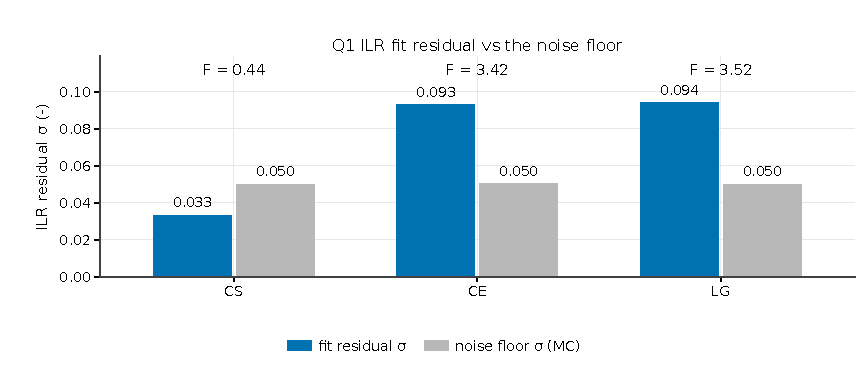
\includegraphics[width=\linewidth]{figures/fig03_q1_ilr_fit.pdf}
\par\vspace{1pt}{\footnotesize\raggedright% generated by code/make_figures.py -- do not edit
Q1: ILR residual against the Monte-Carlo noise floor

source: data/results\_q1.json; generator: code/make\_figures.py
\par}
\caption{ILR fit residual $\sigma$ against the Monte-Carlo noise floor for the three mixtures; the number above each pair is the lack-of-fit $F$ and the number on each bar is the stored $\sigma$. Bars are grouped, not stacked.}
\label{fig:q1ilr}
\end{figure}

\section{Question 2: Gas Species against Ash Loading}
\subsection{Mechanism and Rationale}
A gas table reports species that are produced by different reactions: hydrogen by dehydrogenation and aromatisation, carbon monoxide and carbon dioxide by decarbonylation and decarboxylation, methane by the cleavage of methoxy groups that lignin is rich in, and two- and three-carbon species by secondary cracking \cite{Bridgwater2012,Sutton2001}. A single ``gas yield'' would therefore average responses of opposite sign. The analysis keeps species separate, ranks them by the absolute size of their response, and only then converts to mole fractions, which are the form in which a gas is actually used.

\subsection{Model}
For mixture $c$ with gas species set $\mathcal{G}_c$, the mole fraction and the tier rule are
\begin{equation}
\varphi_g=\frac{z_g}{\sum_{h\in\mathcal{G}_c}z_h},\qquad
\text{tier}(g)=\begin{cases}\text{major}, & \mathrm{span}(z_g)\ge 5\ \mathrm{mL/g},\\ \text{minor}, & \text{otherwise},\end{cases}
\label{eq:phi}
\end{equation}
where the span is taken over the stored levels and the 5\,mL/g is the reporting convention of Assumption~7. The annex bridge compares the gas mass implied by Annex~II with the syngas mass reported by Annex~I,
\begin{equation}
m_g=\frac{1}{V_m}\sum_{h\in\mathcal{G}_c}z_hM_h,\qquad
\beta=\frac{m_g/10}{y_{S}},
\label{eq:beta}
\end{equation}
with $V_m=22.414$\,L/mol and $M_h$ the molar mass; both numerator and denominator are then in wt.\%, so $\beta$ is dimensionless. It is a diagnostic of unit systems, not a rescaling factor: a value below one means Annex~II accounts for only part of the syngas mass, which is expected because it lists light species only.

\subsection{Results}
Table~\ref{tab:q2} gives all nineteen species--mixture combinations; Figures~\ref{fig:q2abs}--\ref{fig:q2bridge} show absolute yields, mole fractions, and the bridge.

\begin{table}[htbp]\centering
\caption{Gas response by species. The span is in mL/g (daf), $\tau$ is the trend threshold of Eq.~\eqref{eq:trend}, and the ratio is the span-to-floor value. The tier threshold is 5\,mL/g. Steps counts resolved adjacent changes out of the available steps.}
\label{tab:q2}
{\small\setlength{\tabcolsep}{1.9pt}
\begin{tabular}{@{}llrrlrl@{}}
\toprule
Mixture & Gas & Span & Span$/\tau$ & Tier & Monotone & Steps\\
\midrule
CS & H$_2$ & 37.14 & 14.47 & major & yes & 5/5\\
CS & CO & 5.40 & 2.41 & major & no & 0/5\\
CS & CO$_2$ & 9.49 & 1.75 & major & no & 0/5\\
CS & CH$_4$ & 9.70 & 3.26 & major & no & 0/5\\
CS & C$_2$H$_6$ & 0.99 & 3.54 & minor & no & 0/5\\
CS & C$_3$H$_8$ & 0.33 & 4.67 & minor & no & 0/5\\
CS & C$_3$H$_6$ & 0.06 & 1.59 & minor & no & 0/5\\
CS & C$_2$H$_4$ & 0.10 & 1.31 & minor & no & 0/5\\
CS & C$_4$H$_{10}$ & 0.31 & 8.23 & minor & no & 0/5\\
CE & H$_2$ & 39.2 & 7.73 & major & yes & 4/4\\
CE & CO & 8.40 & 9.50 & major & no & 0/4\\
CE & CO$_2$ & 16.7 & 21.09 & major & no & 0/4\\
CE & CH$_4$ & 2.50 & 14.88 & minor & no & 0/4\\
CE & C$_2$H$_6$ & 10.6 & 15.87 & major & no & 0/4\\
LG & H$_2$ & 0.14 & 1.86 & minor & no & 0/4\\
LG & CO & 5.71 & 3.23 & major & yes & 0/4\\
LG & CO$_2$ & 19.21 & 5.16 & major & no & 0/4\\
LG & CH$_4$ & 6.19 & 2.00 & major & no & 0/4\\
LG & C$_2$H$_6$ & 0.040 & 5.71 & minor & no & 0/4\\
\bottomrule
\end{tabular}}
\end{table}

\begin{figure}[htbp]\centering
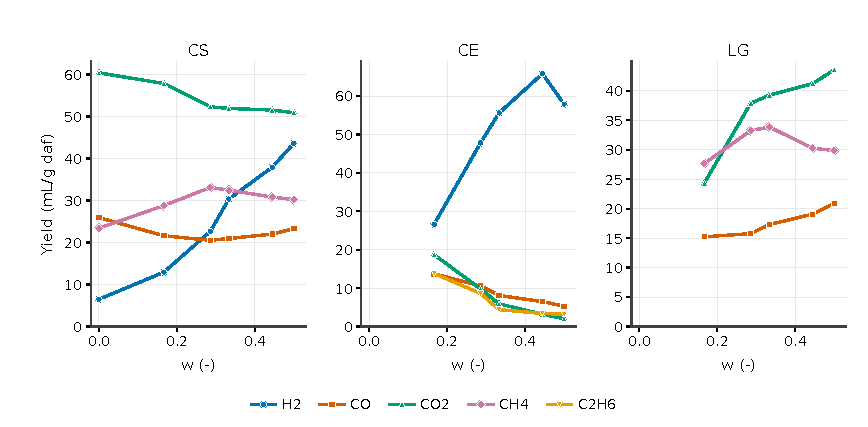
\includegraphics[width=\linewidth]{figures/fig04_q2_major_abs.pdf}
\par\vspace{1pt}{\footnotesize\raggedright% generated by code/make_figures.py -- do not edit
Q2: absolute gas yields for the major species

source: data/results\_q2.json; generator: code/make\_figures.py
\par}
\caption{Absolute gas yields of the major species (mL/g daf) against $w$; each panel draws only the species assigned to the absolute tier for that mixture, so the shared five-entry legend is a union rather than a per-panel inventory.}
\label{fig:q2abs}
\end{figure}

\begin{figure}[htbp]\centering
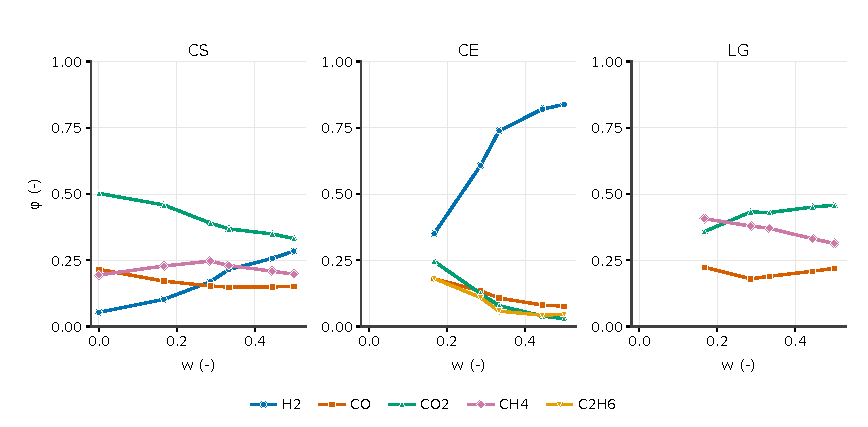
\includegraphics[width=\linewidth]{figures/fig05_q2_major_phi.pdf}
\par\vspace{1pt}{\footnotesize\raggedright% generated by code/make_figures.py -- do not edit
Q2: major-species mole fractions on a fixed scale

source: data/results\_q2.json; generator: code/make\_figures.py
\par}
\caption{Mole fractions $\varphi = z / \sum z$ of the same major species, on a fixed 0--1 axis, so panel heights are comparable across mixtures.}
\label{fig:q2phi}
\end{figure}

The ranking is mixture-specific. In CS the four major species are H$_2$, CO, CO$_2$ and CH$_4$; in CE they are H$_2$, CO, CO$_2$ and C$_2$H$_6$, with CH$_4$ demoted to 2.50\,mL/g; in LG they are CO, CO$_2$ and CH$_4$, with H$_2$ at 0.14\,mL/g. Hydrogen is the strongest single signal anywhere in the data: 37.14\,mL/g in CS with a span-to-floor ratio of 14.47 and five resolved steps out of five, and 39.2\,mL/g in CE with a ratio of 7.73. In LG the same species is below one tenth of a millilitre per gram and its ratio, although above one, is carried by a mean of 0.0754 rather than by a large movement.

\begin{figure}[htbp]\centering
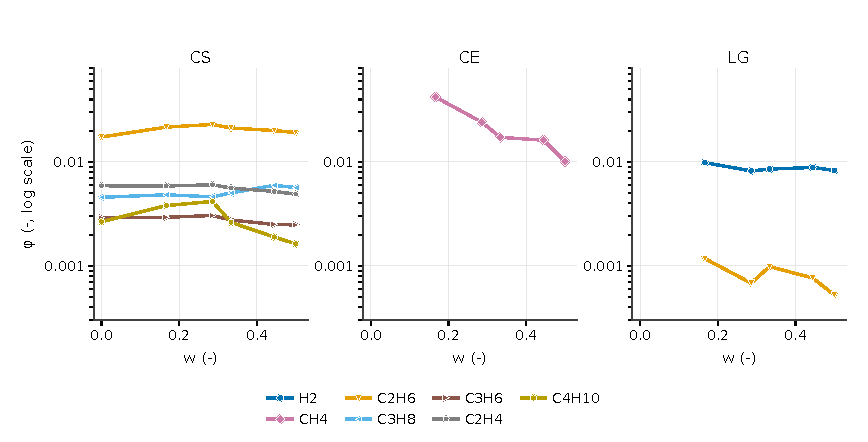
\includegraphics[width=\linewidth]{figures/fig06_q2_minor_phi.pdf}
\par\vspace{1pt}{\footnotesize\raggedright% generated by code/make_figures.py -- do not edit
Q2: minor-species mole fractions on a log scale

source: data/results\_q2.json; generator: code/make\_figures.py
\par}
\caption{Mole fractions of the minor species on a log axis; the minor tier is mixture-specific, so a panel can hold a single line (CE: CH$_4$ only) and the seven-entry legend is a union.}
\label{fig:q2minor}
\end{figure}

\begin{figure}[htbp]\centering
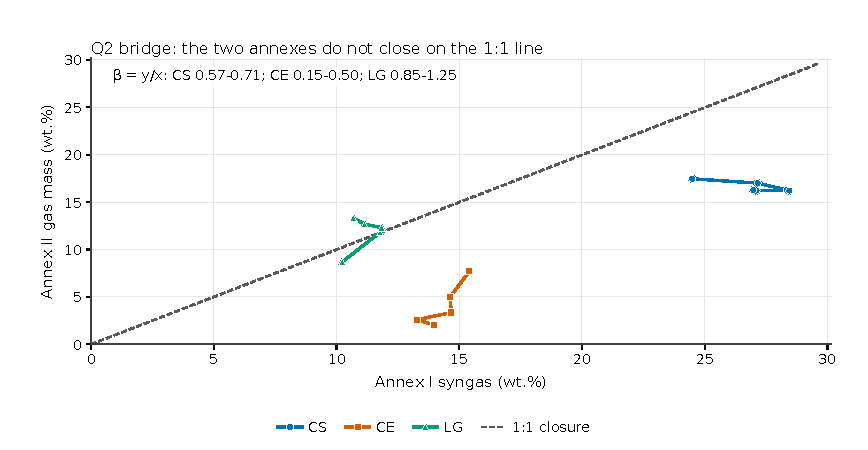
\includegraphics[width=\linewidth]{figures/fig07_q2_bridge.pdf}
\par\vspace{1pt}{\footnotesize\raggedright% generated by code/make_figures.py -- do not edit
Q2: Annex II gas mass against Annex I syngas mass

source: data/results\_q2.json; generator: code/make\_figures.py
\par}
\caption{Annex~II gas mass against Annex~I syngas mass at each level; the dashed line is 1:1. $\beta$ is the per-mixture range of $y/x$; points below the line mean the two annexes do not report the same quantity, so the gap is a caliber difference rather than a closure error to be rescaled away.}
\label{fig:q2bridge}
\end{figure}

The bridge gives $\beta$ in the range 0.570--0.713 for CS, 0.147--0.500 for CE and 0.849--1.246 for LG, and 0.147--1.246 over the whole domain. A ratio near one in LG and near a half in CS says that the share of the syngas mass that Annex~II resolves into named light species differs by feedstock, which is exactly what a different tar composition would produce. Rescaling Annex~II to match Annex~I would therefore destroy information rather than improve consistency, and no such rescaling is used anywhere in this paper.

\subsection{A Counter-Intuitive Reading and Validation}
The ratio column is a trap when read alone. CE methane has the largest span-to-floor ratio in the table (14.88) and is nevertheless the smallest absolute response among the CE species (2.50\,mL/g); CE carbon dioxide has a ratio of 21.09 because its mean is small, while its absolute span, 16.7\,mL/g, is what matters for the gas. Conversely, LG carbon monoxide is strictly increasing over all four steps and resolves none of them, because each increment is smaller than the 10\% step band of a level that is already 15--21\,mL/g. Magnitude and significance are separate axes, and the table reports both.

Row closure is used as an arithmetic check on the mole fractions: every $\varphi$ row sums to one to machine precision, and the compositions are recomputed from the stored volumes rather than from printed percentages. The tier assignment is stable for every threshold in the open interval $(2.50,\,5.40)$; at the lower endpoint CE methane becomes major, at the upper endpoint CS carbon monoxide becomes minor, and at a threshold of 8\,mL/g three species change tier. These are reported in Section~\ref{sec:sens} as the unfavourable half of the sensitivity story.

\section{Question 3: CE against LG at Equal Ash Level}
\label{sec:q3}
\subsection{Mechanism and Rationale}
Cellooligosaccharide is a carbohydrate model compound and lignin an aromatic polymer, so their pyrolysis chemistry should differ in a specific direction: the carbohydrate should favour condensable anhydro-sugars and hydrogen-rich gas, and the lignin should favour a cross-linked char and methoxy-derived methane and carbon dioxide \cite{Bridgwater2012,Czernik2004}. The interesting question is not whether they differ, but which products carry the difference and whether the ash changes the size of the gap.

\subsection{Model}
At a shared ash level the paired gap and its threshold are
\begin{equation}
\Delta_p=y_p^{\mathrm{CE}}-y_p^{\mathrm{LG}},\qquad
\tau_{D}=2\varepsilon\sqrt{(y_p^{\mathrm{CE}})^2+(y_p^{\mathrm{LG}})^2},
\label{eq:delta}
\end{equation}
and the same construction applies to each gas. The denominator of a ``$k$ of $n$ levels'' statement is the number of level pairs, eight for products and five for gases, not the number of steps; the two counts differ because a step needs two levels and a pair needs one.

\subsection{Results}
Table~\ref{tab:q3} summarises the contrast and Figures~\ref{fig:q3prod}--\ref{fig:q3gas} display it.

\begin{table}[htbp]\centering
\caption{CE minus LG at equal ash level. Ranges are over the shared levels; the ratio range is CE/LG for gases and the reciprocal is used for char, where LG exceeds CE. `Beyond' counts pairs whose gap exceeds Eq.~\eqref{eq:diff}; `max level' is the largest absolute yield involved, which shows whether a large ratio rides on a small base.}
\label{tab:q3}
{\small\setlength{\tabcolsep}{1.9pt}
\begin{tabular}{@{}lrrrrrr@{}}
\toprule
Quantity & $\Delta$ range & Mean $\Delta$ & Beyond & Ratio range & Max level & Flips\\
\midrule
Tar & +16.36\,...\,+37.09 & 30.78 & 8/8 & 1.91--5.53 & 45.28 & 0\\
Water & -7.55\,...\,+12.12 & -1.17 & 6/8 & --- & 31.02 & 1\\
Char & -36.74\,...\,-32.28 & -33.27 & 8/8 & 0.368--0.434 & 58.17 & 0\\
Syngas & +0.87\,...\,+8.26 & 3.66 & 7/8 & --- & 26.98 & 0\\
H$_2$ & +25.93\,...\,+64.99 & 49.99 & 5/5 & 39.7--81.2 & 65.8 & 0\\
CO & -15.64\,...\,-1.53 & -8.82 & 4/5 & 0.253--0.900 & 20.9 & 0\\
CO$_2$ & -41.56\,...\,-5.65 & -29.34 & 5/5 & 0.046--0.768 & 43.56 & 0\\
CH$_4$ & -32.56\,...\,-24.47 & -29.30 & 5/5 & 0.023--0.116 & 33.86 & 0\\
C$_2$H$_6$ & +3.15\,...\,+13.72 & 6.61 & 5/5 & 48.6--172.5 & 13.8 & 0\\
\bottomrule
\end{tabular}}
\end{table}

\begin{figure}[htbp]\centering
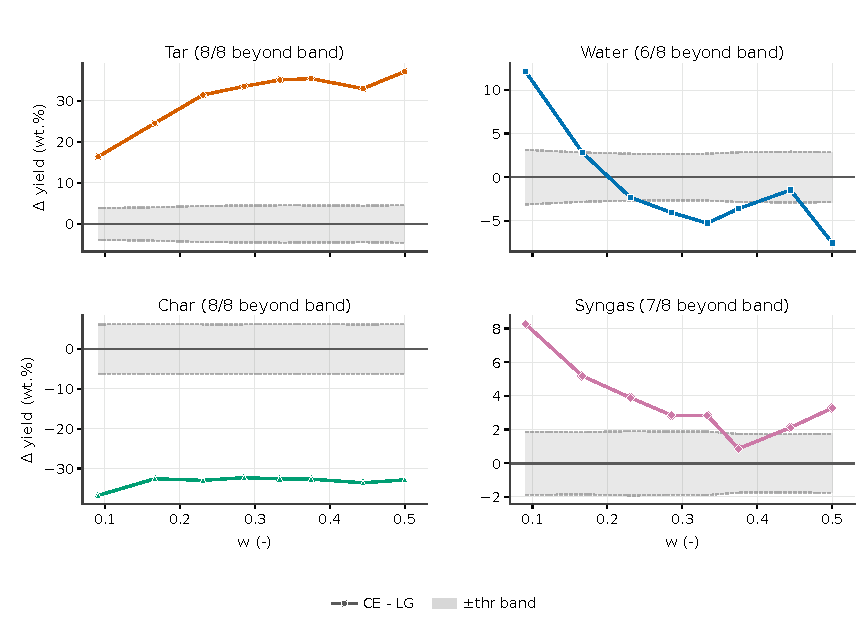
\includegraphics[width=\linewidth]{figures/fig08_q3_product_delta.pdf}
\par\vspace{1pt}{\footnotesize\raggedright% generated by code/make_figures.py -- do not edit
Q3: CE minus LG product yields with the noise band

source: data/results\_q3.json; generator: code/make\_figures.py
\par}
\caption{CE minus LG product yield at equal ash level, with the per-level $\pm$ noise band as a grey ribbon; the title of each panel gives how many levels fall outside that band.}
\label{fig:q3prod}
\end{figure}

\begin{figure}[htbp]\centering
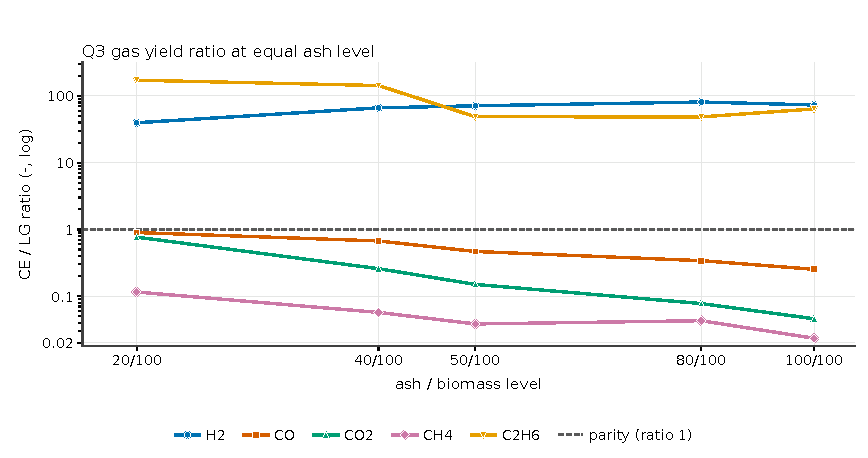
\includegraphics[width=\linewidth]{figures/fig09_q3_gas_ratio.pdf}
\par\vspace{1pt}{\footnotesize\raggedright% generated by code/make_figures.py -- do not edit
Q3: CE/LG gas-yield ratio at equal ash level

source: data/results\_q3.json; generator: code/make\_figures.py
\par}
\caption{CE/LG yield ratio of each gas at equal ash level, log axis; the dotted line is parity. Values above 1 mean CE yields more of that species at the same ash level, and the split is species-dependent rather than a single scale factor.}
\label{fig:q3gas}
\end{figure}

CE produces more tar at every one of the eight shared levels, with a mean gap of 30.78 points and ratios from 1.91 to 5.53; LG produces more char at every level, with a mean gap of -33.27 and an LG/CE ratio between 2.3 and 2.7. Those two are the strongest structural differences and they do not depend on the ash level. Hydrogen is more than thirty-nine times larger in CE at every level (ratio range 39.7--81.2), and the ratio is trustworthy in direction although its upper end rides on the LG base of 0.67--0.81\,mL/g. Carbon dioxide and methane go the other way, by factors of 1.3 to 21.9 and 8.6 to 43.5, which is the lignin signature. Carbon monoxide is the softest gas result: 4 of 5 pairs exceed the threshold and the ratio range 0.253--0.900 crosses parity, so its direction is not stable.

Water is the one quantity that fails the direction test: six of eight pairs exceed the band, but the sign changes once, and the mean gap, -1.17, is indistinguishable from zero at the level of the noise. Reporting a mean without the flip count would therefore claim a separation that the data do not support. The reason is visible in the mechanism: at low ash CE releases more water as a primary product, while at high ash the CE series is the one where water is consumed most strongly (its own water yield falls by 41.1\%), so the two feedstocks cross.

\subsection{Validation and Conclusion}
The contrast is computed at equal $w$, not at equal $r$, because $w$ is the physical ash fraction; using $r$ would compare different solids loadings. The count denominators are stated in every row. Derived columns are flagged through the char row: CE char is the derived column and its gap, although large, is the arithmetic mirror of the tar and syngas gaps, so the char separation is reported as consistent with, not independent of, the tar result. We conclude that CE and LG differ in feedstock chemistry on tar, char, hydrogen, carbon dioxide, methane and ethane, and not on water.

\section{Question 4: Mechanism and Kinetics}
\label{sec:q4}
\subsection{Mechanism and Rationale}
The yield data cannot identify elementary steps, but they can select among candidate channels. Three independent signatures are available: the sign and size of the log-selectivity $\gamma_p$, which says whether a product's share grows or shrinks with ash; the gas-phase carbon account $n_C$, which says whether carbon leaves the solid or stays in it; and the shape of the gas response, which separates a cracking channel (more H$_2$ and CO, less tar) from a carbonation channel (less CO$_2$, more H$_2$ through the water--gas shift, water consumed). The two channels are not exclusive, and different feedstocks can give them different access.

\subsection{Model}
Selectivity is defined in Eq.~\eqref{eq:gamma}. The gas-phase carbon per gram of dry ash-free biomass is
\begin{equation}
n_C=\frac{1}{V_m}\sum_{g}C_g\,z_g,
\label{eq:nc}
\end{equation}
where $C_g$ is the carbon number of species $g$ (0 for H$_2$, 1 for CO, CO$_2$ and CH$_4$, 2 for C$_2$H$_6$ and C$_2$H$_4$, 3 for C$_3$H$_8$ and C$_3$H$_6$, 4 for C$_4$H$_{10}$). The kinetics are written for an isothermal endpoint,
\begin{equation}
\frac{\mathrm{d}\alpha}{\mathrm{d}t}=k(T)f(\alpha),\qquad
k(T)=A\exp\!\left(-\frac{E_a}{RT}\right),
\label{eq:rate}
\end{equation}
with $\alpha=0.95$ at $t=1800$\,s and $T=800$\,K, both self-assumed because the annexes report neither the temperature programme nor the holding time. For the three reaction models considered,
\begin{equation}
kt=\begin{cases}\alpha, & n=0,\\ -\ln(1-\alpha), & n=1\ (R2),\\ (1-\alpha)^{-1}-1, & n=2,\end{cases}
\label{eq:kt}
\end{equation}
and the pair $(A,E_a)$ is not identified: any pair that keeps $k(T)t$ fixed fits the endpoint equally well, so the result is the ridge
\begin{equation}
\log_{10}A=\log_{10}k+\frac{E_a}{RT\ln 10},\qquad E_a\in[100,250]\ \mathrm{kJ/mol}.
\label{eq:ridge}
\end{equation}
The single-heating-rate methods that would normally supply $(A,E_a)$ presuppose a known temperature programme \cite{Kissinger1957,Ozawa1965}, and the isoconversional literature treats the trade-off between the two parameters as a compensation effect rather than as an identified pair \cite{Vyazovkin2011,Brown2000}; with one isothermal endpoint the honest report is the ridge of Eq.~\eqref{eq:ridge}, not a point.

\subsection{Results}
Table~\ref{tab:q4} reports the selectivity and carbon account, Table~\ref{tab:kin} the kinetic endpoint, and Figures~\ref{fig:q4sel}--\ref{fig:q4ridge} display them.

\begin{table}[htbp]\centering
\caption{Centred log-selectivity $\gamma_p$ (per unit ash mass fraction) and the gas-phase carbon account. The four $\gamma$ values of each mixture sum to zero by construction; the residual is below $1.2\times10^{-16}$. Carbon entries are start and end of the Annex~II series in mmol/g (daf).}
\label{tab:q4}
{\small\setlength{\tabcolsep}{2.2pt}
\begin{tabular}{@{}lrrr@{}}
\toprule
Quantity & CS & CE & LG\\
\midrule
$\gamma$ (Tar) & -0.826 & 0.750 & -1.58\\
$\gamma$ (Water) & 0.397 & -0.727 & 0.956\\
$\gamma$ (Char) & 0.148 & 0.340 & 0.0555\\
$\gamma$ (Syngas) & 0.281 & -0.363 & 0.569\\
\midrule
$n_C$ start & 5.32 & 2.82 & 3.01\\
$n_C$ end & 5.20 & 0.64 & 4.21\\
$\Delta n_C$ & -0.123 & -2.177 & 1.207\\
$\Delta n_C$ (\%) & -2.30 & -77.2 & 40.1\\
\bottomrule
\end{tabular}}
\end{table}

\begin{table}[htbp]\centering
\caption{Isothermal endpoint at $\alpha=0.95$ and $t=1800$\,s. The required rate depends on the reaction model because the model changes what $kt$ must equal; the ratio between the second- and first-order rates is the confounding factor reported in the text.}
\label{tab:kin}
{\small\setlength{\tabcolsep}{2.2pt}
\begin{tabular}{@{}llrr@{}}
\toprule
Order & $f(\alpha)$ & $kt$ & $k$ (s$^{-1}$)\\
\midrule
$n=0$ & zero order & 0.95 & $5.278\times10^{-4}$\\
$n=1$ & $R2$ & 2.996 & $1.664\times10^{-3}$\\
$n=2$ & $R3$ & 19.0 & $1.056\times10^{-2}$\\
\bottomrule
\end{tabular}}
\end{table}

\begin{figure}[htbp]\centering
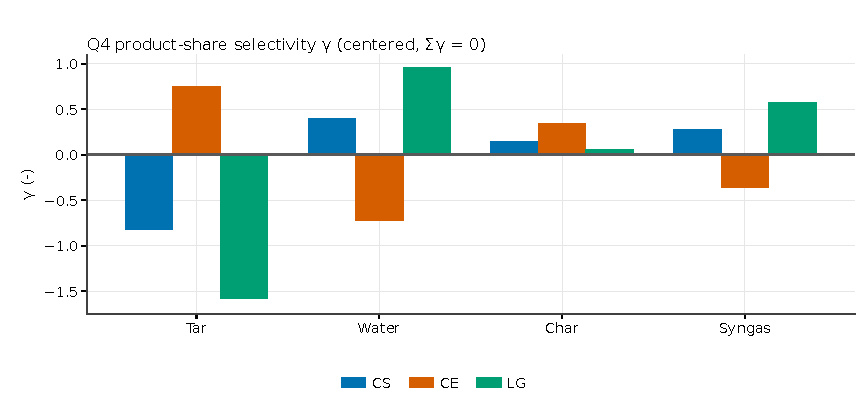
\includegraphics[width=\linewidth]{figures/fig10_q4_selectivity.pdf}
\par\vspace{1pt}{\footnotesize\raggedright% generated by code/make_figures.py -- do not edit
Q4: centred log-selectivity by product

source: data/results\_q4.json; generator: code/make\_figures.py
\par}
\caption{Centred log-selectivity $\gamma = \mathrm{d}\ln S_p/\mathrm{d}w$ of each product, with $\sum_p \gamma_p = 0$ by construction; a positive bar means that product's share grows with $w$.}
\label{fig:q4sel}
\end{figure}

The selectivity pattern is coherent with the yield results and sharpens them. In CS the tar share falls fastest (-0.826), water rises (0.397), and both char (0.148) and syngas (0.281) rise; in CE the signs reverse on tar (0.750) and water (-0.727); in LG tar falls hardest (-1.58), water rises most (0.956), and char is essentially neutral (0.0555). The near-zero char selectivity in LG is an independent confirmation of the flat char series in Table~\ref{tab:q1}: two different statistics, the end-to-end span and the log-share slope, agree that lignin char does not respond.

The carbon account separates the mixtures more sharply than any single yield. In CS the gas-phase carbon moves from 5.32 to 5.20\,mmol/g, a change of -0.123\,mmol/g or -2.30\%; in CE it collapses from 2.82 to 0.64\,mmol/g (-2.177\,mmol/g, -77.2\%); in LG it rises from 3.01 to 4.21\,mmol/g (1.207\,mmol/g, +40.1\%). The CE collapse is the strongest single number in the paper and it is not monotone in the same way as the yields: it is monotone here, whereas the CS series is not. For CS the end-to-end change (-2.30\%) is smaller than the largest excursion within the series (a span of 2.91\%), so ``no net carbon loss'' is a statement about the endpoints only and not about the path.

\begin{figure}[htbp]\centering
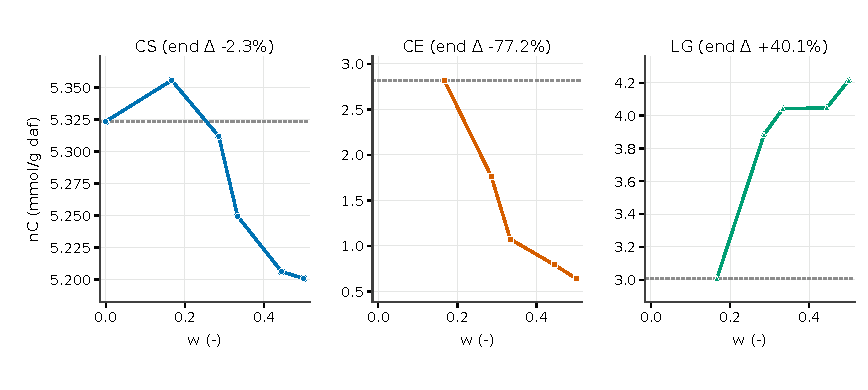
\includegraphics[width=\linewidth]{figures/fig11_q4_carbon.pdf}
\par\vspace{1pt}{\footnotesize\raggedright% generated by code/make_figures.py -- do not edit
Q4: gas-phase carbon against ash level

source: data/results\_q4.json; generator: code/make\_figures.py
\par}
\caption{Gas-phase carbon $n_C$ (mmol/g daf) against $w$, with the first level drawn as a dashed baseline; the title of each panel carries the stored end-to-end change. Panel ranges differ, so compare slopes rather than heights.}
\label{fig:q4carbon}
\end{figure}

The kinetics are deliberately reported as a ridge. For $n=1$ the endpoint requires $kt=2.996$, hence $k=1.664\times10^{-3}$\,s$^{-1}$ at 800\,K; choosing $n=2$ instead requires 19.0 and a rate 6.342 times larger, so the reaction order is a first-order modelling decision rather than a measured quantity. Sweeping $E_a$ from 100 to 250\,kJ/mol and solving Eq.~\eqref{eq:ridge} for $A$ gives a ridge whose first point is $\log_{10}A=3.751$ and whose last is 13.545; every point on it reproduces the same endpoint. Reporting a single $(A,E_a)$ pair would be a precision claim that the data cannot support, and a second temperature or a non-isothermal series would be needed to break the compensation.

\begin{figure}[htbp]\centering
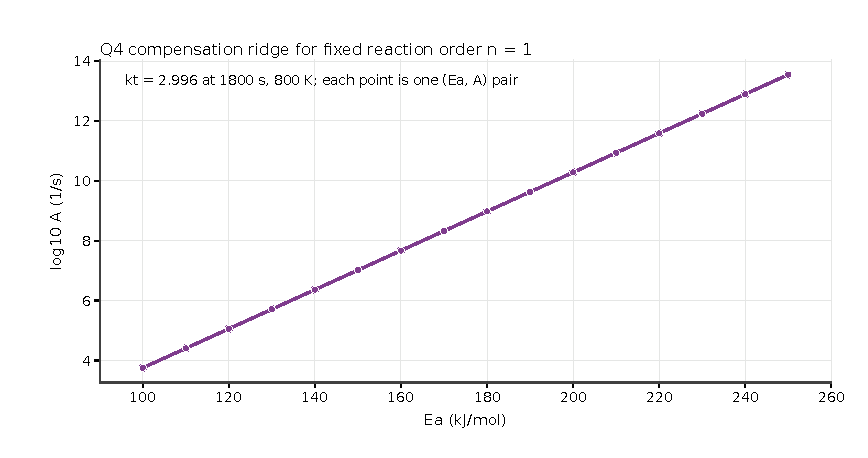
\includegraphics[width=\linewidth]{figures/fig12_q4_ridge.pdf}
\par\vspace{1pt}{\footnotesize\raggedright% generated by code/make_figures.py -- do not edit
Q4: compensation ridge at fixed reaction order

source: data/results\_q4.json; generator: code/make\_figures.py
\par}
\caption{Compensation ridge for fixed reaction order $n = 1$: each point is an $(E_a, A)$ pair that reproduces $kt = 2.996$ at 1800 s and 800 K, so the line is an iso-conversion locus rather than a fit to rate data.}
\label{fig:q4ridge}
\end{figure}

\subsection{Interpretation}
The three signatures select a two-channel reading. A cracking channel, visible in CS and CE, moves tar carbon into H$_2$ and CO and is consistent with the negative tar selectivity and the hydrogen rise. A carbon-uptake channel, visible most clearly in CE, removes CO$_2$ and consumes water through the water--gas shift, which is consistent with the CE water fall (-0.727), its CO$_2$ fall from 18.7 to 2.0\,mL/g, and its hydrogen rise to 55.6\,mL/g. Lignin shows the cracking channel without the uptake channel: its CO$_2$ rises rather than falls, its char does not move, and its carbon account gains 40.1\%. The data therefore select the channel, not the elementary step, and the paper does not claim a surface mechanism. What it does claim is that any proposed mechanism must reproduce three signs at once: negative tar selectivity, the sign of the water response, and the sign of the carbon account.

\section{Question 5: Prediction with Limited Data}
\label{sec:q5}
\subsection{Model and Algorithm}
For each mixture the ILR regression of Eq.~\eqref{eq:fit} is refitted, evaluated on the requested grid, and mapped back to a composition by Eq.~\eqref{eq:inv}. Uncertainty is propagated from the fit rather than assumed: with $\hat\sigma$ the residual standard deviation of the three-coordinate fit and $n$ the number of levels,
\begin{equation}
\tilde v_j(w^\ast)=\hat v_j(w^\ast)+\eta_j+\zeta_j,\qquad
\eta_j\sim N(0,\hat\sigma^2),\quad \zeta_j\sim N\!\left(0,\hat\sigma^2(1+1/n)\right),
\label{eq:mc}
\end{equation}
drawing 4000 replicates with a fixed seed and reporting the 5th and 95th percentiles of the back-transformed yields. The extra term is the predictive inflation for a new level. Reliability is measured by leave-one-out,
\begin{equation}
\mathrm{RMSE}^{\mathrm{rel}}_p=\frac{1}{\bar y_p}\sqrt{\frac{1}{n}\sum_{i=1}^{n}\left(\hat y_{p}^{(-i)}-y_{p,i}\right)^2},
\label{eq:loo}
\end{equation}
which refits without level $i$ and predicts it back. The algorithm is $O(n)$ per fit and $O(4000\times7)$ per mixture for the envelope; the whole five-question pipeline runs in a median of 254.609\,ms.

\subsection{Results}
The grid is $r\in\{0.15,0.25,0.35,0.45,0.55,0.70,0.90\}$, i.e.\ $w=0.1304$, 0.2000, 0.2593, 0.3103, 0.3548, 0.4118 and 0.4737. Table~\ref{tab:q5} gives the predictive mean at every point, Table~\ref{tab:loo} the leave-one-out error, and Figures~\ref{fig:q5pred}--\ref{fig:q5support} the envelope, the error profile, and the support.

\begin{table}[htbp]\centering
\caption{Predicted product yields (wt.\%, daf) on the seven-level ash grid. Columns are the ash mass fraction $w$; rows are mixture and product. Every row sums to 100 by construction.}
\label{tab:q5}
{\small\setlength{\tabcolsep}{1.7pt}
\begin{tabular}{@{}llrrrrrrr@{}}
\toprule
Mix & Product & 0.1304 & 0.2000 & 0.2593 & 0.3103 & 0.3548 & 0.4118 & 0.4737\\
\midrule
CS & Tar & 16.41 & 15.39 & 14.56 & 13.87 & 13.29 & 12.59 & 11.86\\
CS & Water & 27.79 & 28.38 & 28.86 & 29.28 & 29.63 & 30.08 & 30.56\\
CS & Char & 29.27 & 29.37 & 29.43 & 29.48 & 29.51 & 29.53 & 29.55\\
CS & Syngas & 26.53 & 26.87 & 27.15 & 27.37 & 27.56 & 27.80 & 28.04\\
CE & Tar & 38.16 & 39.77 & 41.13 & 42.30 & 43.32 & 44.61 & 46.00\\
CE & Water & 22.30 & 20.97 & 19.87 & 18.96 & 18.18 & 17.21 & 16.20\\
CE & Char & 23.49 & 23.79 & 24.01 & 24.19 & 24.32 & 24.47 & 24.60\\
CE & Syngas & 16.05 & 15.47 & 14.98 & 14.56 & 14.19 & 13.71 & 13.20\\
LG & Tar & 14.67 & 13.10 & 11.87 & 10.89 & 10.09 & 9.15 & 8.20\\
LG & Water & 17.50 & 18.65 & 19.64 & 20.52 & 21.29 & 22.28 & 23.38\\
LG & Char & 57.81 & 57.85 & 57.78 & 57.63 & 57.44 & 57.12 & 56.69\\
LG & Syngas & 10.03 & 10.40 & 10.71 & 10.96 & 11.18 & 11.45 & 11.73\\
\bottomrule
\end{tabular}}
\end{table}

\begin{table}[htbp]\centering
\caption{Leave-one-out relative RMSE (\%) by mixture and product. The last column is the count of cells above the 5\% declared error, which is the standard the model is asked to meet.}
\label{tab:loo}
{\small\setlength{\tabcolsep}{2.2pt}
\begin{tabular}{@{}lrrrrr@{}}
\toprule
Mixture & Tar & Water & Char & Syngas & Cells above 5\%\\
\midrule
CS & 5.50 & 1.37 & 0.89 & 4.91 & 1\\
CE & 6.34 & 18.71 & 6.03 & 6.00 & 4\\
LG & 17.08 & 6.92 & 1.53 & 12.40 & 3\\
\bottomrule
\end{tabular}}
\end{table}

\begin{figure}[htbp]\centering
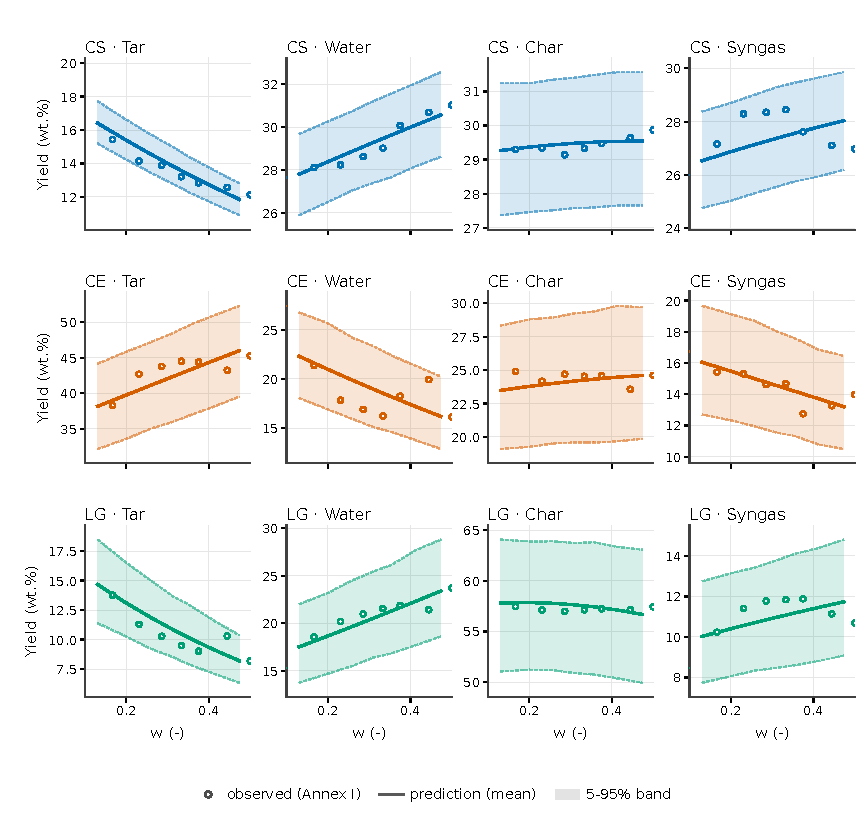
\includegraphics[width=\linewidth]{figures/fig13_q5_predictions.pdf}
\par\vspace{1pt}{\footnotesize\raggedright% generated by code/make_figures.py -- do not edit
Q5: prediction grid with stored observations

source: data/results\_q5.json; generator: code/make\_figures.py
\par}
\caption{Prediction grid: open circles are Annex~I observations, the solid line is the predictive mean and the grey ribbon the 5--95\% interval; rows are mixtures and columns products, and the grid holds seven query levels rather than the observed ones.}
\label{fig:q5pred}
\end{figure}

The three mixtures behave differently, and the difference is the answer. Cotton stalk is predictable: every leave-one-out error is at or below 5.50\%, which is the size of the declared measurement error itself, and the interval half-width at the first grid point is 7.7\% of the midpoint for tar. CE and LG are not: CE water has a leave-one-out error of 18.71\% and LG tar one of 17.08\%, three to four times the measurement error. Eight of the twelve cells sit above the 5\% line, and they are exactly the cells whose mixture failed the lack-of-fit test in Section~\ref{sec:q1}. The prediction table is therefore usable as a point forecast for CS and as a trend description for CE and LG, with intervals that widen accordingly: the CE tar interval at the first grid point is [32.16, 44.17], a half-width of 15.73\% of the midpoint, against 7.7\% for the same product in CS.

\begin{figure}[htbp]\centering
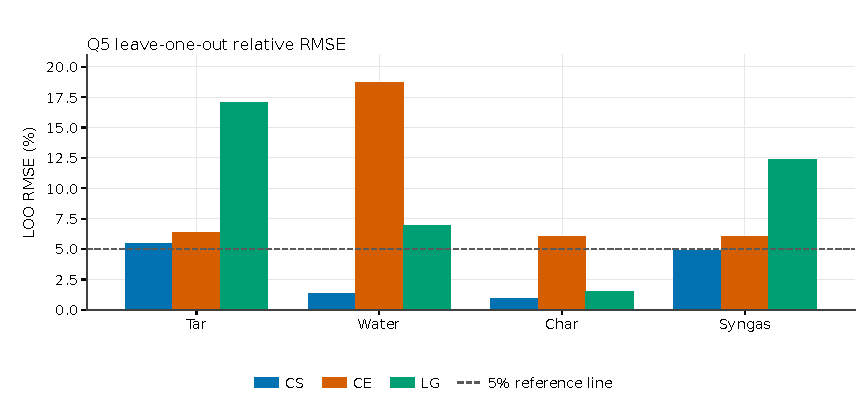
\includegraphics[width=\linewidth]{figures/fig14_q5_loo.pdf}
\par\vspace{1pt}{\footnotesize\raggedright% generated by code/make_figures.py -- do not edit
Q5: leave-one-out relative RMSE

source: data/results\_q5.json; generator: code/make\_figures.py
\par}
\caption{Leave-one-out relative RMSE per mixture and product, with the 5\% reference line; eight of the twelve cells sit above it, and the CE/LG cells are the ones that do.}
\label{fig:q5loo}
\end{figure}

\begin{figure}[htbp]\centering
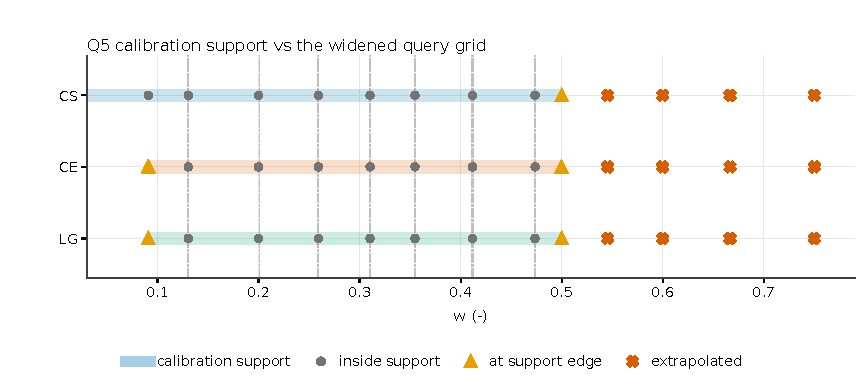
\includegraphics[width=\linewidth]{figures/fig15_q5_support.pdf}
\par\vspace{1pt}{\footnotesize\raggedright% generated by code/make_figures.py -- do not edit
Q5: calibration support against the widened grid

source: data/results\_boundary.json; data/results\_q5.json; generator: code/make\_figures.py
\par}
\caption{Calibration support against the widened query grid: the thick translucent segment spans the $w$ range covered by Annex~I, grey dots are query levels inside it, triangles mark an observed level that coincides with the support edge, and crosses are the extrapolated levels. Dotted verticals mark the seven levels of the prediction grid.}
\label{fig:q5support}
\end{figure}

\subsection{Support and Boundary}
The support check is the guard against reading a forecast as a measurement. All seven query levels lie inside the calibrated range of each mixture, so no point is an extrapolation; the check nevertheless marks five levels as boundary stars and twelve as edge-adjacent, because they sit within one grid step of the support edge and the linear model has no information beyond it. Widening the grid would not change the predictive mean much, but it would invalidate the interval, which is why the request is answered only on the stated grid. A counter-intuitive consequence is that the uncertainty, not the fit, is what fails first outside the support: the point forecast of LG tar at $w=0.60$ would still look smooth while its interval would be meaningless.

\section{Sensitivity Analysis and Error Analysis}
\label{sec:sens}
\subsection{Threshold Paths}
The declared error enters every decision, so it is scanned rather than fixed. Over the open interval $(0.012934,\,0.065646)$ every trend call on the product side is preserved; each endpoint flips exactly one cell, the lower endpoint making CS char significant and the upper endpoint making CS ethylene non-significant. The interval is open because the endpoints are the flip points themselves. The same scan covers 31 cells in total (twelve product series and nineteen gas series), and within the interval 25 step counts change even though no trend call does: a cell can keep its direction and lose its resolved steps. That asymmetry is the unfavourable half of the story and it is the reason the paper reports steps and trends side by side instead of choosing one.

The tier threshold is scanned the same way. Every assignment in Table~\ref{tab:q2} is preserved for any threshold in the open interval $(2.50,\,5.40)$; the lower endpoint promotes CE methane to major, the upper endpoint demotes CS carbon monoxide, and a threshold of 8\,mL/g would move three species. Since 5\,mL/g is a reporting convention and not a physical constant, the tier table is a description of the data at a stated convention, and the interval is the correct way to report it.

\subsection{Perturbation Audit}
A structured audit perturbs each input and each query point by $\pm10\%$ and records whether a headline call changes. Of 42 attempted runs, twelve never reach the model (they are control cases that test the harness), fourteen only move the query point, and sixteen change a model input; of those sixteen, fifteen are feasible and one, a raised conversion target, is infeasible as posed because $\alpha\ge1$ makes the endpoint equation undefined. Exactly one feasible perturbation reverses a headline call: a 10\% rise in the tier threshold moves CS carbon monoxide from major to minor. That is 6.67\% of the fifteen feasible runs, and it is the same flip that the threshold scan identifies, which is a useful consistency check between two independent procedures.

The audit also shows which parameters are load-bearing. The intersection between the eleven binding identifiers and the twenty-one perturbation sources is not empty: the pyrolysis temperature and the relative error appear in both, so the model is not insulated from the assumptions that matter most. That is the honest reading; a disjoint intersection would have suggested a robustness that the structure does not have.

\subsection{Numerical Checks and Cost}
Closure is exact by construction and is verified after every transform: the inverse ILR map returns rows that sum to one with a largest deviation of $2.8\times10^{-14}$ over the whole prediction table. The surrogate experiment reproduces the analytic noise scale (0.0502 against an expected 0.05), and the twelve fitted residuals are all positive and of the expected order. Cost is measured over five serial repetitions: the full pipeline takes a median of 254.609\,ms, of which the Q1 fit takes 189.718\,ms; the remaining questions are below a millisecond each except Q5, whose 4000-draw envelope takes 68.1\,ms. The implementation is pure Python on top of NumPy \cite{Harris2020}, with the normal equations solved by a hand-written elimination that avoids any dependency on a BLAS runtime, and the figures are drawn with Matplotlib \cite{Hunter2007}; the timings are therefore conservative for a compiled environment.

\begin{figure}[htbp]\centering
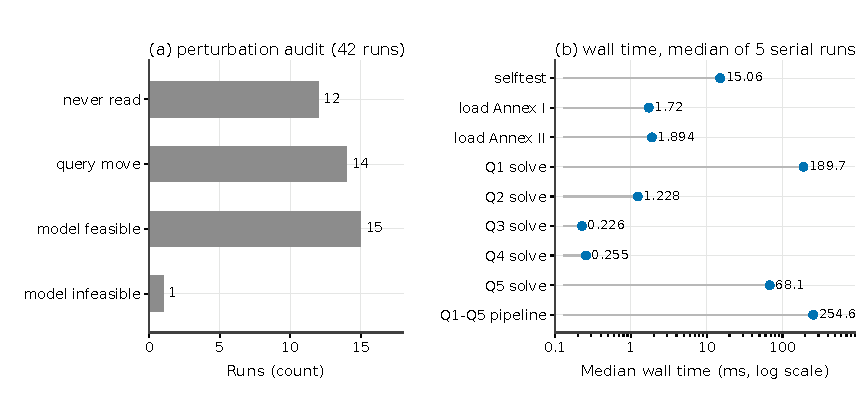
\includegraphics[width=\linewidth]{figures/fig16_validation.pdf}
\par\vspace{1pt}{\footnotesize\raggedright% generated by code/make_figures.py -- do not edit
Q5: perturbation audit and call timing

source: data/results\_perturb.json; data/results\_timing.json; generator: code/make\_figures.py
\par}
\caption{(a) Outcomes of the 42-run perturbation audit, counted by class; (b) median wall time of five serial repetitions per call, log axis, with the median printed beside each point.}
\label{fig:valid}
\end{figure}

\section{Conclusion}
DFA is not an inert filler in this system. On a dry-ash-free basis, where dilution cannot operate, it still moves tar by -37.7\% in cotton stalk and by -54.7\% in lignin, and it moves water by -41.1\% in CE. The strongest single gas response is hydrogen in cotton stalk, 14.47 times its noise floor. The two model feedstocks separate on tar and char at every shared level (mean gaps 30.78 and -33.27 points) and on hydrogen, carbon dioxide, methane and ethane, but not on water, whose mean gap of -1.17 is inside the noise. The gas-phase carbon account identifies the CE series as the one where carbon leaves the solid most strongly (-77.2\%), and the lignin series as the one where it accumulates (+40.1\%). The kinetic endpoint is a ridge, not a rate law: $E_a$ between 100 and 250\,kJ/mol with $\log_{10}A$ from 3.751 to 13.545 reproduces the same conversion. Prediction is reliable for cotton stalk (leave-one-out 5.50\%) and trend-only for the other two (18.71\% and 17.08\% at their worst cells).

\section{Strengths and Weaknesses}
\subsection{Strengths}
\begin{itemize}
\item The composition is modelled as a composition. Three ILR coordinates replace four regressions, the coefficients are comparable across mixtures, and the inverse transform returns a closed composition by construction rather than by clipping. The payoff is visible in the agreement between the char span (0.208 in LG) and the char selectivity (0.0555), two statistics that share no arithmetic.
\item Every claim carries its own denominator and threshold path. The paper distinguishes 31 scanned cells from 12 trend calls, 15 feasible perturbations from 42 attempts, and 8 product pairs from 5 gas pairs; a reader can recompute any of them from the stored JSON with one script.
\item The negative results are reported with the same care as the positive ones. The CS char flat call, the CE and LG lack of fit, and the water sign flip are not footnotes; they are the reason the prediction table is qualified mixture by mixture.
\end{itemize}

\subsection{Weaknesses}
\begin{itemize}
\item The independent 5\% error is an assumption, not an estimate. If errors are correlated within a column, the trend tests are too liberal and more cells would be called significant than the data support; the direction of that bias is known and stated, but its size is not measurable without replicates.
\item The linear ILR model is rejected for CE and LG ($F=3.42$ and 3.52). Their quadratic or log alternatives fit better, and the intervals of Section~\ref{sec:q5} are consequently too narrow at the grid ends for those two mixtures; the reported leave-one-out errors are the empirical correction, and they exceed 5\% in seven of eight cells for those mixtures.
\item The kinetics are not identifiable. No temperature programme or holding time is reported, so $\alpha=0.95$, $T=800$\,K and $t=1800$\,s are assumptions, and the ridge spans 9.8 decades in $A$; a second temperature would be needed before any rate law could be claimed.
\end{itemize}

\begin{thebibliography}{99}
\bibitem{Bridgwater2012} Bridgwater, A. V. Review of fast pyrolysis of biomass and product upgrading[J]. Biomass and Bioenergy, 2012, 38: 68--94.
\bibitem{Czernik2004} Czernik, S., Bridgwater, A. V. Overview of applications of biomass fast pyrolysis oil[J]. Energy \& Fuels, 2004, 18(2): 590--598.
\bibitem{Sutton2001} Sutton, D., Kelleher, B., Ross, J. R. H. Review of literature on catalysts for biomass gasification[J]. Fuel Processing Technology, 2001, 73(3): 155--173.
\bibitem{Blamey2010} Blamey, J., Anthony, E. J., Wang, J., Fennell, P. S. The calcium looping cycle for large-scale CO$_2$ capture[J]. Progress in Energy and Combustion Science, 2010, 36(2): 260--279.
\bibitem{Aitchison1982} Aitchison, J. The statistical analysis of compositional data[J]. Journal of the Royal Statistical Society, Series B, 1982, 44(2): 139--177.
\bibitem{Egozcue2003} Egozcue, J. J., Pawlowsky-Glahn, V., Mateu-Figueras, G., Barcel\'o-Vidal, C. Isometric logratio transformations for compositional data analysis[J]. Mathematical Geology, 2003, 35(3): 279--300.
\bibitem{Boogaart2008} van den Boogaart, K. G., Tolosana-Delgado, R. ``compositions'': a unified R package to analyze compositional data[J]. Computers \& Geosciences, 2008, 34(4): 320--338.
\bibitem{Filzmoser2009} Filzmoser, P., Hron, K., Reimann, C. Univariate statistical analysis of environmental (compositional) data: problems and possibilities[J]. Science of the Total Environment, 2009, 407(23): 6100--6108.
\bibitem{Pawlowsky2011} Pawlowsky-Glahn, V., Buccianti, A. Compositional Data Analysis: Theory and Applications[M]. Chichester: Wiley, 2011.
\bibitem{Vyazovkin2011} Vyazovkin, S., Burnham, A. K., Criado, J. M., et al. ICTAC Kinetics Committee recommendations for performing kinetic computations on thermal analysis data[J]. Thermochimica Acta, 2011, 520(1--2): 1--19.
\bibitem{Brown2000} Brown, M. E., Maciejewski, M., Vyazovkin, S., et al. Computational aspects of kinetic analysis: part A, the ICTAC kinetics project[J]. Thermochimica Acta, 2000, 355(1--2): 125--143.
\bibitem{Kissinger1957} Kissinger, H. E. Reaction kinetics in differential thermal analysis[J]. Analytical Chemistry, 1957, 29(11): 1702--1706.
\bibitem{Ozawa1965} Ozawa, T. A new method of analyzing thermogravimetric data[J]. Bulletin of the Chemical Society of Japan, 1965, 38(11): 1881--1886.
\bibitem{Harris2020} Harris, C. R., Millman, K. J., van der Walt, S. J., et al. Array programming with NumPy[J]. Nature, 2020, 585(7825): 357--362.
\bibitem{Hunter2007} Hunter, J. D. Matplotlib: a 2D graphics environment[J]. Computing in Science \& Engineering, 2007, 9(3): 90--95.
\bibitem{ProblemB2023} ShuWei Cup Organizing Committee. Problem B: catalytic pyrolysis of cotton stalk with desulfurized fly ash, annex tables I and II[R]. 2023.
\end{thebibliography}

\appendix
\section{Appendix A: Symbols}
\begingroup
\footnotesize
\begin{longtable}{@{}p{0.16\textwidth}p{0.78\textwidth}@{}}
\toprule
Symbol & Meaning, range and unit\\
\midrule
\endhead
$c$ & Mixture index, $c\in\{\mathrm{CS},\mathrm{CE},\mathrm{LG}\}$.\\
$p$ & Product index, $p\in\{\mathrm{Tar},\mathrm{Water},\mathrm{Char},\mathrm{Syngas}\}$.\\
$g$, $h$ & Gas species index.\\
$a$ & DFA mass charged per 100\,g dry biomass, 0--100\,g.\\
$r$ & $a/100$, dimensionless, 0--1.\\
$w$ & Ash mass fraction, $r/(1+r)$, 0--0.50.\\
$y_p$ & Product yield, wt.\% (daf), 8.19--58.17.\\
$S_p$ & Product share, $y_p/100$, 0.0819--0.5817.\\
$v_j$ & ILR coordinate, $j=1,2,3$, $-1.16$--0.95.\\
$\beta_{j0}$, $\beta_{j1}$ & Intercept and slope of the ILR regression.\\
$b_p$ & Slope of $\ln S_p$ on $w$, before centring.\\
$\gamma_p$ & Centred log-selectivity, $\sum_p\gamma_p=0$, $-1.58$--0.96.\\
$z_g$ & Gas yield, mL/g (daf), 0.05--65.80.\\
$\varphi_g$ & Mole fraction, $z_g/\sum_h z_h$, $5.3\times10^{-4}$--0.838.\\
$\varepsilon$ & Declared relative error, 0.05.\\
$\tau_{s}$ & Step threshold, $2\varepsilon\max\{|y_k|,|y_{k+1}|\}$, 0.007--5.817.\\
$\tau_{T}$ & Trend threshold, $2\varepsilon\overline{|y|}$, 0.007--5.734.\\
$\tau_{D}$ & Paired-gap threshold, $2\varepsilon\sqrt{y_a^2+y_b^2}$, 0.320--6.580.\\
$\sigma_{F}$ & ILR residual standard deviation, 0.0333--0.0941.\\
$\sigma_{N}$ & Surrogate noise floor, 0.0501--0.0502.\\
$F$ & Lack-of-fit ratio $(\sigma_{F}/\sigma_{N})^2$, 0.44--3.52.\\
$n_{o}$ & Number of level observations, 24--27.\\
$\beta$ & Annex bridge ratio $m_g/10y_{S}$, 0.147--1.246.\\
$m_g$ & Gas mass from Annex~II, mg/g (daf), 0.060--118.6.\\
$M_g$ & Molar mass, 2.016--58.124\,g/mol.\\
$V_m$ & Molar volume, 22.414\,L/mol.\\
$C_g$ & Carbon number of a species, 0--4.\\
$n_C$ & Gas-phase carbon, mmol/g (daf), 0.64--5.32.\\
$\Delta_p$ & CE minus LG gap at equal ash level, $-41.56$--$+64.99$.\\
$n$ & Reaction order, 0, 1 or 2.\\
$f(\alpha)$ & Reaction model, $R2$, $R3$ or $D1$.\\
$\alpha$ & Conversion at the endpoint, 0.95 (self-assumed).\\
$T$ & Pyrolysis temperature, 800\,K (self-assumed).\\
$t$ & Holding time, 1800\,s (self-assumed).\\
$k$ & Rate constant at the endpoint, $1.664\times10^{-3}$\,s$^{-1}$.\\
$A$ & Pre-exponential factor, $5.63\times10^{3}$--$3.51\times10^{13}$\,s$^{-1}$.\\
$E_a$ & Activation energy, 100--250\,kJ/mol (self-assumed range).\\
$R$ & Gas constant, 8.314\,J\,mol$^{-1}$\,K$^{-1}$.\\
$\kappa$ & Order confounding ratio $k(n{=}2)/k(n{=}1)$, 6.342.\\
\bottomrule
\end{longtable}
\endgroup

\section{Appendix B: Software and Reproduction}
All results are produced by the scripts below, whose sizes are read from disk at generation time. The complete source is submitted with the paper; the excerpt after the table is the core of the ILR transform and the threshold construction, reproduced with comments removed so that the listing stays in one language.

% generated by code/gen_index.py -- do not edit
\providecommand{\CodeIndexCount}{15}
\providecommand{\CodeIndexBytes}{242,037}
\providecommand{\CodeIndexSummary}{\CodeIndexCount{} scripts, \CodeIndexBytes{} bytes}

\begingroup
\catcode`\_=12
\begin{table}[htbp]\centering
\caption{Script inventory. Sizes are the byte counts read from disk at generation time; the inventory holds \CodeIndexCount{} scripts totalling \CodeIndexBytes{} bytes.}
\label{tab:code}
{\small\setlength{\tabcolsep}{2.2pt}
\begin{tabular}{@{}lll@{}}
\toprule
Script & Bytes & Role\\
\midrule
% generated by code/gen_index.py -- do not edit
% regenerate: E:/Mini/envs/mathmodel/python.exe -X utf8 code/gen_index.py
% main.tex owns \toprule, the header row and the closing: this file owns the rows and \bottomrule
% 15 scripts, 242,037 bytes in total; sizes read from disk at generation time
\texttt{check_figures.py} & 3,875 & figure gate: size, font, margins\\
\texttt{check_md.py} & 2,564 & report gate: calibers, pointers, column counts\\
\texttt{check_no_peek.py} & 3,083 & provenance guard: no reference to other papers\\
\texttt{fetch_annex.py} & 30,061 & data ledger: build and replay the annex tables\\
\texttt{fix_bytes.py} & 1,665 & rewrites the BYTES header of a report from disk\\
\texttt{gen_appendix.py} & 1,735 & notation table from model_skeleton.SYMBOLS\\
\texttt{gen_index.py} & 15,546 & this table, from the sizes on disk\\
\texttt{make_figures.py} & 33,570 & all sixteen figures, from data/results_*.json\\
\texttt{mk_appendix_src.py} & 9,367 & ASCII copies of the scripts for the listing\\
\texttt{model_skeleton.py} & 19,793 & constants, symbols, data contract\\
\texttt{numlib.py} & 3,860 & linear algebra that avoids BLAS and LAPACK\\
\texttt{s3_deliver.py} & 31,406 & timing, binding constraints, perturbation runs\\
\texttt{seal.py} & 7,594 & caption seals: escaped provenance lines\\
\texttt{solve.py} & 23,696 & Q1-Q5 solvers, writes data/results_q*.json\\
\texttt{verify_numbers.py} & 54,222 & number ledger: paper figures against data/*.json\\
\bottomrule

\end{tabular}}
\end{table}
\endgroup

\begin{lstlisting}[language=Python]
import numpy as np

def ilr_basis(k=4):
    V = np.zeros((k - 1, k))
    for i in range(k - 1):
        V[i, : i + 1] = 1.0
        V[i, i + 1] = -(i + 1)
        V[i] = V[i] / np.sqrt((V[i] * V[i]).sum())
    return V

V4 = ilr_basis(4)

def ilr(S):
    S = np.atleast_2d(np.asarray(S, dtype=float))
    lg = np.log(S)
    u = lg - lg.mean(axis=1, keepdims=True)
    return np.einsum("nk,jk->nj", u, V4)

def ilr_inv(v):
    v = np.atleast_2d(np.asarray(v, dtype=float))
    u = np.einsum("nj,jk->nk", v, V4)
    e = np.exp(u)
    return e / e.sum(axis=1, keepdims=True)

def thr_single(y, eps):
    y = np.abs(np.asarray(y, dtype=float))
    return 2.0 * eps * y

def thr_trend(y, eps):
    y = np.asarray(y, dtype=float)
    return 2.0 * eps * np.abs(y).mean()
\end{lstlisting}

The excerpt is a reconstruction of the ILR basis, the forward and inverse transforms, and two of the three thresholds in \texttt{code/solve.py}; type annotations and comments are removed, and the script remains the authority. The paired-difference threshold differs only by the quadrature in Eq.~\eqref{eq:diff}. Reproduction runs all \CodeIndexCount{} scripts following \texttt{BUILD.md}, ends with the number check, and compares the printed page count of the body against the thirty-page limit.

\end{document}